\documentclass[12pt, a4paper, twoside]{report}
\usepackage[utf8]{inputenc}
\usepackage{tabularx}
\usepackage{placeins}
\usepackage{wrapfig}
\usepackage[newfloat]{minted}
\usepackage{graphicx}
\graphicspath{{images/}}

\usepackage{amsmath}
\usepackage{parskip}
\usepackage{hyperref}
\usepackage{parcolumns}
\usepackage{algpseudocode}
\usepackage[ruled]{algorithm}
\usepackage[sorting=none]{biblatex}
\addbibresource{cite.bib}

\usepackage{fancyhdr}
\pagestyle{fancy}
\renewcommand{\chaptermark}[1]{\markboth{\MakeUppercase{#1}}{}}
\fancyhead{}
\fancyhead[RO, LE]{\leftmark}

\usepackage{listings}
\lstdefinestyle{mystyle}{
    basicstyle=\small,
    language=C,
    numberstyle=\tiny,
    numbers=left,                    
    numbersep=5pt
}
\lstset{style=mystyle}

\providecommand{\keywords}[1]
{
  \small	
  \textbf{\textit{Keywords---}} #1
}

\usepackage{titlesec}
\titleformat{\chapter}{\bf\huge}{\thechapter.}{20pt}{\huge\bf}

\usepackage{epigraph}
\setlength\epigraphwidth{.7\textwidth}
\setlength\epigraphrule{0pt}

%\renewcommand{\familydefault}{\sfdefault}
\renewcommand{\topfraction}{.75}
\renewcommand{\floatpagefraction}{.8}%

\begin{document}

\title{
{Concurrent Datastructure Design for\\ Software Transactional Memory} \\
\vspace{1cm}
{\large Vrije Universiteit Amsterdam} \\ 
{\large Bachelor Project} \\
\vspace{1.3cm}
{
\includegraphics[height=28mm]{vu-griffioen.pdf}}}

\author{Daniel Köves \\
        \texttt{\href{mailto:d.koves@student.vu.nl}{d.koves@student.vu.nl}}\vspace*{0.5cm}\\
\setlength{\tabcolsep}{12pt}
\begin{tabular}{c c}
  {\normalsize Supervisor}   & {\normalsize Second reader}  \\
  {\normalsize Prof. Wan Fokkink}   & {\normalsize Dr. Thilo Kielmann}
\end{tabular}
}


\date{June 2021}

\maketitle

\pagenumbering{roman}
\tableofcontents

\listoffigures

\newpage


\begin{abstract}
\thispagestyle{plain}
\setcounter{page}{4}
The following paper set out to investigate how transactional memory can be applied to concurrent datastructure design. Specifically, how it can provide a clean and accessible interface in replacement of locks and built on top of lock-free primitives for concurrent algorithms. Two of such datastructures are implemented, a transactional Red-Black Tree and a Skiplist, with underlying encounter-order and commit-time transactions taking care of concurrent insertions. Results show that word-based commit-time transactions cannot be successfully applied to Red-Black Trees without imposing an unnatural design on the datastructure, due to the fact that the commit-time transaction's write-list consist of (address, value) 2-tuples that are oblivious to chain of dependencies between the writes. For Skiplists, no such restrictions exist, with both encounter-order and commit-time transactions exhibiting optimal scaling properties. As opposed to findings of other papers like \cite{tl, tl2}, which promote the use of the commit-time mechanism for high-contention, this paper finds that due to the large amount of aborting transactions, which are expected in case of high-contention, and the more expensive commit-time API operations, the encounter-order locking mechanism outperforms commit-time locking on all metrics with a factor of two. Furthermore, it can be empirically concluded that the use of the transactional algorithm design is much less error-prone than its lock based counterpart, without further restrictions on its structure posed by lock-free primitives. While performance-wise, hand-crafted concurrent datastructures might prove to be more effictive, the transactional design can open up the process to a wider range of programmers by providing a straight-forward abstraction for concurrency.

\keywords{transactional memory, concurrent datastructures, parallelization}
\end{abstract}

\pagenumbering{arabic}
\chapter{Introduction}
\epigraph{"He who controls the spice controls the universe."}{---Frank Herbert, \textit{Dune}}

\section{Background}
In the era of multi- and many-core systems, achieving parallelisation to a sufficiently high degree is of great importance. Speeding up sequential applications by parallelising them or consciously designing highly concurrent programs has been a goal in computing for some time now to fully utilise the available machine architectures and infrastructure. However, this attempt comes with a catch. In the 1960s, Gene Amdahl presented a theoretical upper bound\cite{amdahl} on the speedup of parallelised programs. It roughly states that even if a small amount of the program remains sequential (i.e. cannot be parallelised), the maximum achievable speedup will be rather limited. As an example, consider a program of which $75\%$ can be fully parallelised and denote this fraction with $p$, and let $s = 1 - p$ be the remaining sequential work. The theoretical speedup $S(n)$, where $n$ is the number of cores available, will than be no bigger than $S(n) \leq \lim_{n \to \infty} 1/(s + p/n) = 4$. With $p = 0.9$, the theoretical speedup bound is still only 10, even if we have an infinite number of processing cores available. In real-world applications, the implications of Amdahl's Law is not as daunting as it may first seem. Firstly, it assumes that the application operates on fixed problem size. However, today's massively concurrent machines allow computations on much larger datasets in the same amount of time. The argument that parallelisation is not just about speeding up programs but enabling them to deal with larger datasets is captured by Gustafson's Law\cite{gustafson}. Both Amdahl's Law and Gustafson's Law, however, fail to take communication into consideration. As systems get more and more complicated, so does the inherent complexity of communication between them; therefore, both laws paint a somewhat simplistic picture. Still, the main implication of both is that there are inherent limitations to parallelisation and that introducing $n$ more computing cores does not immediately result in $n$-fold speedup.

Another problem involving concurrent programming is achieving synchronisation. Synchronisation refers to how separate concurrent \textit{threads} manage and operate on shared data, i.e. ideally want maximum performance while ensuring that no concurrent operations overwrite each other or see inconsistent states. One of the more simple ways to achieve this is by using \textit{locks}. Consider for example the simple \textit{spinlock} with two operations: \texttt{lock()} and \texttt{unlock()}. Spinlocks (or locks in general) can be thought of as some global variable that threads acquire before executing operations on shared data. Those operations are said to reside in the \textit{critical section}. If one thread wants to operate on a shared datastructure, it must first acquire the lock, perform the operations and then release the lock. In the meanwhile, other threads wishing to perform their work on the shared datastructure \textit{spin}, until they can acquire the lock. One (of the many) problems with this simple way of achieving synchronisation, often referred to as \textit{coarse-grained locking} is that it is slow and does not scale well to highly concurrent applications. When the computation runs on many threads, even if they want to modify completely disjoint parts of a potentially large datastructure, they must wait in line to perform their actions. Therefore, computation is still sequential, even though many computing cores are available. A possible alternative is to use \textit{fine-grained locking} by associating certain parts of the datastructure with their own locks. That way, more concurrent threads can operate on different parts of the data. This can even be further enhanced and complicated by using \textit{readers-writers} locks, i.e. when each locked part of the datastructure is associated with two locks; one must be acquired for reading the object while the other must be acquired when writing the object. 

The above description about locks, by no means complete, is already quite complex and is still far from the whole picture. Mainly, it does not take into account how threads are scheduled by the operating system. Scheduling algorithms are \textit{non-deterministic}, which, when applied to algorithms, generally means that given the same input, the algorithm might produce different outputs. Therefore, we cannot make any assumptions on how a thread is scheduled or when it is preempted or descheduled. This creates a problem for locking: \textit{priority-inversion} happens when a lower-priority thread is preempted while holding onto a lock that a higher-priority thread needs. This means that the higher-priority thread needs to wait for the lower-priority one to be rescheduled and release the lock. Moreover, in datastructures where locks must be acquired one-after-another (also called \textit{hand-over-hand locking}) to reach a certain part of the structure, \textit{convoying} can occur, which means that if a thread further down the chain is delayed, all other threads behind it need to wait as well. \textit{Deadlock} occurs when threads try to acquire the same locks in a different order and execution grinds to a halt.

A possible way to move away from locks is the use of \textit{lock-free} primitives that are also detailed in Section \ref{subsection:sync}. Hardware operations like \textit{compare-and-swap} work by only allowing operations on shared data to succeed if the current value that a thread reads matches the actual value of the object (i.e. no other thread modified it in the meanwhile). These primitives, however, still have limitations and problems. Firstly, they usually operate on a single word in memory; therefore, only one location can be modified \textit{atomically} (i.e. inseparably). Moreover, by this limitation, more complex lock-free algorithms tend to have a very unnatural structure.

What might be a solution to the problems described above? On the one hand, locks are performant; however, there are inherent problems with them. Apart from priority-inversion, convoying, and deadlocks, generally speaking, programming with locks is hard as complex situations can arise that are difficult to debug. Lock-free primitives propose an alternative; however, more complex algorithms tend to have an unnatural structure to them due to the limitations of the primitives.

A potential solution is \textit{transactional memory}, a concept introduced by Herlihy and Moss in 1993\cite{herlihy-moss}. Transactions, which are already an established phenomenon in databases, are a set of instructions operating on some shared data which have the properties that they are \textit{serialisable} and \textit{atomic}. Serializability means that transactions appear to execute one after another and never seem to interleave. Atomicity indicates that transactions make speculative changes to memory which they only make atomically visible by \textit{committing} if no inconsistencies are found (i.e. no other transaction modified the shared data that the transaction accessed in the meanwhile). Suppose there is a conflict, the transaction aborts and can retry executing its operations. This provides a nice abstraction away from the "dirty details" of concurrent algorithms, as it is the transactional runtime system that takes care of the hard work. Wrapping instructions in transactions that modify a shared datastructure and retrying them until they are able to commit also provides a sufficiently straightforward interface, without the need to worry about locking, priority-inversion or unnaturally structured complex algorithms.

\section{Goals}
The goals of the paper are to present the history of transactional memory and, specifically, how it can be applied to concurrent datastructure design. Designing concurrent datastructures usually involve hand-crafting them to certain use cases, and the process involved is very demanding - often best left to experts. Using the transactional approach, however, the paper would like to show that designing transactional datastructures is not much different from designing sequential ones. In cases when the application performance isn't critical, the transactional interface can offer a very accessible approach to dealing with concurrency. The paper proposes two of such transactional datastructures that will be detailed in Section \ref{section:trb} and \ref{section:skip}. Finally, an experiment is described in Chapter \ref{chapter:eval} to investigate the performance of certain transactional memory implementations underlying the datastructures and answer the research questions outlined below.

\section{Research Questions}
In order to realise the goals of the paper, the following research questions are explored related to transactional datastructure design:

\begin{enumerate}
    \item How does the locking scheme of lock-based STM implementations affect the insertion performance of concurrent red-black trees and skiplists?
    \item How well suited is transactional programming for concurrent datastructures in terms of ease-of-design?
\end{enumerate}

Research Question 1 is explored thoroughly in Chapter \ref{chapter:eval}, where the proposed STM implementations are tested on two transactional datastructures: a Red-Black Tree and Skiplist.

Research Question 2 is a follow-up and a minor one, where based on the results described in Section \ref{section:res} further conclusions on the ease of transactional design can be drawn.

\section{Organisation}
The rest of the paper is organised as follows: Chapter 2 introduces common concepts and terminology regarding progress conditions and synchronisation primitives. Chapter 3 gives an overview of Transactional Memory both in hardware and software by presenting a handful of papers and their approaches. Chapter 4 details the implementations proposed by the paper, including two STM versions: one using encounter-order locking, the other using commit-time locking. Moreover, two transactional datastructures, a red-black tree and a skiplist, are described. Chapter 5 describes the evaluation of the implementations and presents and discusses the results. Finally, Chapter 6 gives the concluding remarks of the paper with possible future directions to explore.

\chapter{Terminology}
This section aims to give an overview of the terminology used throughout the paper. Firstly, progress conditions are detailed, i.e. different implementation strategies concerning concurrent methods of an object. Then, the idea behind the two most common lock-free hardware synchronisation primitives is described.

\section{Progress Conditions}
Progress conditions describe different ways an object's method implementation can act on concurrent pending invocations. A method implementation is said to be \textbf{non-blocking} if threads are able to make progress even when one thread is delayed\cite{book}. An implementation is \textbf{blocking} if delaying one thread can prevent others from making progress\cite{book}.

\subsection{Non-blocking progress conditions}
A method implementation is \textbf{wait-free} if a thread with a pending invocation to such a method keeps taking steps, it will finish in a finite number of steps. This guarantees that every thread makes progress if it takes steps\cite{book}. In practice, this is often inefficient and wait-freedom can be relaxed in multiple ways.

One such way is to settle for \textbf{lock-free} methods which require that only some threads make progress that has a pending invocation to a lock-free method of an object. This guarantees that the whole system makes progress, even though some thread might be delayed.

Another way to relax the wait-free condition is to guarantee progress under certain assumptions on how the threads are scheduled. A method implementation is \textbf{obstruction-free} if it is guaranteed that a thread finishes in a finite number of steps after any point it executes \textit{in isolation}, i.e. in a period when no other threads take steps.

\subsection{Blocking progress conditions}
When relaxing the non-blocking property, the following grouping can be made. A method implementation is \textbf{starvation-free} if a thread is guaranteed to complete in a finite number of steps when all other threads with pending invocations are making progress.

Finally, a method implementation is \textbf{deadlock-free}, whenever there is an invocation to that method and all threads with invocations are making progress, \textit{some} will finish in a finite number of steps\cite{book}.

\section{Hardware Synchronisation}
\label{subsection:sync}
To achieve synchronisation, most modern processor architectures provide one of the two following primitives: the \textit{Compare-and-Swap} or \textit{Load-link/Store-conditional} instructions.

\subsection{Compare-and-Swap}
Compare-and-Swap (or \textit{CAS} for short), shown in Algorithm \ref{alg:cas}, is an instruction that takes three parameters: an address $\mathcal{A}$ in memory, and expected value $\mathcal{E}$ and an new value $\mathcal{V}$ for for that address. Compare-and-Swap executes \textit{atomically} the following actions: in case address $\mathcal{A}$ contains $\mathcal{E}$, $\mathcal{A}$ is updated to $\mathcal{V}$ and true is returned. Else, nothing is changed and false is returned. 

\begin{algorithm}
\label{alg:cas}
\caption{\textit{boolean atomically} CAS($\mathcal{A}, \mathcal{E}, \mathcal{V}$)}
\begin{algorithmic}[1]
    \If {*$\mathcal{A} = \mathcal{E}$}
        \State *$\mathcal{A} \gets \mathcal{V}$
    \Else
        \State \Return false
    \EndIf
    \State \Return true
\end{algorithmic}
\end{algorithm}

An interesting inherent problem of this approach, known as the ABA problem, occurs when two concurrently executing threads try to modify the same location. Consider the scenario when thread $T_1$ reads location $\mathcal{L}$ and sees that its current value is $A$. Thread $T_1$ is preempted and thread $T_2$ is allowed to execute. Thread $T_2$ reads location $\mathcal{L}$, modifies its value to $B$, and then back to $A$ after doing some work. When thread $T_1$ is scheduled back, it sees that the value of location $\mathcal{L}$ has not changed and continues executing. The execution scenario can prove to be incorrect, since thread $T_1$ is unaware of the undetected change of values to $B$ (and potentially other side effects of that action) at location $\mathcal{L}$.
 
\subsection{Load-link/Store-conditional}
Another way to achieve synchronisation, which does not pose ABA-like issues, is with a pair of instructions Load-link \texttt{LL} and Store-conditional \texttt{SC}. The \texttt{LL} instruction loads the value stored in address $\mathcal{A}$. Subsequent \texttt{SC} call to that address with a new value $\mathcal{V}$ succeeds only if the value of $\mathcal{A}$ has not changed since the corresponding \texttt{LL} call. The \texttt{SC} instruction fails if the value at $\mathcal{A}$ has changed since the \texttt{LL} call; therefore, also detecting the ABA problem.

\chapter{Literature Review}
This section gives an overview of the history of \textit{Transactional Memory}, starting from Herlihy and Moss' 1993 paper, in which the term was coined\cite{herlihy-moss}. Following it, \textit{Software Transactional Memory} is presented through multiple proposed versions like the original non-blocking implementation of Shavit and Touitou\cite{shavit-stm}, Herlihy's DSTM\cite{DSTM} and Fraser's OSTM\cite{OSTM, ostm2}. Finally, the proposed \textit{blocking} implementations are detailed with attention to Ennals' STM\cite{ennals-stm}, but also the \textit{Transactional Locking I \& II} algorithms proposed by Shavit et al.\cite{tl, tl2}.

\section{Hardware Transactional Memory}

\textit{Transactional Memory} was introduced to the distributed computing world by Herlihy and Moss in 1993\cite{herlihy-moss}. In their paper, the authors detailed a new multi-processor architecture providing lock-free synchronization, which would enable programmers to specify read-modify-write operations on several words in memory, via transactions. It is implemented as an extension to already existing cache-coherence protocols, and require specialised hardware support in terms of instructions such as \texttt{LT} "Load-transactional", \texttt{ST} "Store-transactional", etc\cite{herlihy-moss}. Their proof of concept describes transactions as a \textit{serializable} and \textit{atomic} finite sequence of instructions. Serializability refers to the fact that transactions appear to happen one after another and they never appear to interleave. Atomicity indicates that transactions make tentative changes to shared memory and either \textit{commit}, by making its changes atomically visible to other transactions or \textit{abort}, by discarding its changes\cite{herlihy-moss}.\par

\section[Non-blocking Software Transactional Memory]{Non-blocking Software Transactional\\Memory}
\subsection{STM of Shavit et al.}
In 1996, Shavit and Touitou proposed an alternative transactional memory design which is implemented entirely in software, called \textit{Software Transactional Memory}\cite{shavit-stm} (or \textit{STM} for short). Their design builds on top of that of Herlihy and Moss, however, it can also be implemented on existing machines with \textit{Load-link/Store-conditional} operations\cite{shavit-stm}. The paper focuses on implementing \textit{static transactions}, where the data set is known in advance, and therefore, each transaction can be viewed as an atomic procedure storing the given new values\cite{shavit-stm}. Their STM implementation is also \textit{non-blocking}, which means that a thread is guaranteed to make progress even when other threads are suspended.

Implementation wise, the original STM approach was as follow. Two shared datastructures coordinate the processes and their transactions: a vector \texttt{Memory} of size M which contains every transactional memory block, and a vector \texttt{Ownership} of the same size pointing to \textit{records} that determine which transaction owns a certain block of memory. Records are shared structures that store information about the current transaction its corresponding process started. 

When executing a transaction, a process's record is initialised and status set to \textit{stable}. Afterwards, ownership for all involved locations of the dataset needs to be acquired in some increasing order. If that succeeds, the transaction writes the old values to the locations' records, calculates the new values and writes them to the memory locations, and finally, sets its status to \textit{success}. If the ownerships cannot all be acquired, the transaction sets its status to \textit{failure, failadd} where \textit{failadd} is the address for which the ownership couldn't be acquired\cite{shavit-stm}. In case of a failed transaction, the algorithm utilises a \textit{cooperative method} to help the other transaction holding ownership of the location needed for the failed transaction. This is done as follows: if the failed transaction is not already a \textit{helping transaction}, it first releases all ownerships that it previously acquired and helps the transaction that holds ownership to the location which failed by becoming a helper for that transaction\cite{shavit-stm}.

\subsection{Herlihy's DSTM}
Whereas the original STM algorithm of Shavit and Touitou was \textit{static}, where the transactions and memory usage is known in advance\cite{shavit-stm}, the first \textit{dynamic} Software Transactional Memory implementation was proposed by Herlihy et al. in 2003, known as \textit{DSTM}\cite{DSTM}. The algorithm allows dynamic creation of transactions and transactional objects, moreover, transactions can determine their course of action based on previously read (transactional) values, which makes it suitable to operate on dynamic datastructures\cite{DSTM}. It inherits the \textit{non-blocking} and \textit{lock-free} properties, i.e. a suspended thread will not prevent others from advancing. 

The algorithm described in the paper is originally implemented in \texttt{Java} and its workings can be described as follows. The \textit{DSTM} algorithm operates on \textit{transactional objects} which are accessed by transactions. These transactional objects are a wrapper around conventional objects, which can be modified by first \textit{opening} the transactional objects and modifying its contents\cite{DSTM}. These changes are only \textit{speculative}, i.e. they have no observable effect until the transaction commits. The interface the authors provided consist of the following: firstly, the \texttt{TMThread} class represents transactional threads, which is implemented as a wrapper around \texttt{Java}'s thread class. The thread class holds a status field which can either be \texttt{ACTIVE}, \texttt{COMMITTED} or \texttt{ABORTED}. Secondly, the \texttt{TMObject} class represents transactional objects accessed by the threads, which can be opened in \texttt{READ} or \texttt{WRITE} modes. Each transactional type must have the \texttt{TMCloneable} interface implemented which provides a \texttt{clone()} method used for speculative modification\cite{DSTM}. 

After a transaction begins, it must call \texttt{open()} with an appropriate mode on the transactional objects it wishes the change. This creates a working copy of the object (using the before-mentioned \texttt{clone()} method) which the transaction can safely modify, called the \textit{version} of the object. Each thread maintains a read-table of opened objects. The version of an object is determined by the status of the transaction that last opened it in \texttt{WRITE} mode. The \texttt{TMObject} class holds a reference to a \texttt{Locator} object, which in turn holds two versions of each object and a reference to the transaction that last opened it in \texttt{WRITE} mode. If that transaction commits, the \textit{new} version of the object becomes valid, else the \textit{old} version. The level of indirection by introducing the \texttt{Locator} object in between an object's metadata and its contents is necessary to be able to atomically change the three field of the \texttt{Locator}, and therefore, the \texttt{TMObject} itself. This is performed by swinging the reference in the \texttt{TMObject} class to a new \texttt{Locator}\cite{DSTM}. After each open call, the transaction is \textit{validated}, to ensure that the accessed object's \textit{version} is not outdated yet, i.e. another transaction hasn't committed and modified the object in the meanwhile. This is performed by checking each entry in the read-only table and confirming that the local version of an object is still the latest committed version of the object and that the transaction is still active and has not been aborted\cite{DSTM}. Committing a transaction involves validating its read-table and using a \textit{CAS} operation to change its status from \texttt{ACTIVE} to \texttt{COMMITTED}\cite{DSTM}.

\subsection{Fraser's OSTM}
The STM implementation proposed by Fraser in \cite{OSTM} and summarised by Fraser and Harris in \cite{ostm2} titled \textit{OSTM} for \textit{object-based} STM, shares some of the key elements of Herlihy et al.'s \textit{DSTM}\cite{DSTM}. 

The algorithm is both \textit{obstruction-free} and operates on \textit{objects} as the unit of concurrency, which contain \textit{references} that can be opened for transactional access\cite{OSTM}. Each transaction maintains \textit{read-only} and \textit{read-write} linked-lists of \textit{object handles} which point to \textit{object-headers}. These headers are used to point to the most recent version of an object that is accessed by a transaction. When an object of opened from write access, a \textit{shadow copy} of the object is created. The shadow copy is used to make tentative changes to an object, which will become visible to the application upon successful commit\cite{OSTM}.

Transactional commits contain two phases: the \textit{acquire} and \textit{release} phases. In the acquire phase, each opened object's header must be acquired in some efficient order, by replacing the object handles with the transactions \textit{descriptor}. If a header is already acquired by another transaction, that transaction is aided to finish\cite{OSTM}. After the acquire phases, based on its outcome, the transaction's status is changed atomically to either successful or aborted. On success, in the \textit{release} phase, each object has its header swinged to its shadow copy by a \textit{Compare-and-Swap} operation\cite{OSTM}.

Three issues are mentioned by the authors with the current design. Firstly, in order to avoid a performance bottleneck when opening objects for read access on datastructures where there is a single entry point, the algorithm only acquires headers for objects in the read-write list which is followed by a \textit{read} phase. In the read phase, the algorithm checks whether the version of an object in its read-only list matches that of the object when it was first opened. In case they do, the algorithm can commit, else it must abort\cite{OSTM}.

Secondly, in some cases, an object may be updated after the read phase, but before the transaction status is updated and its changes are visible. To avoid this, transactions report a new status \textit{read-checking} in their read phase and ensuring that the transaction is such a phase atomically commit or abort. This is done by helping a transaction in its read phase reach its \textit{decision point}, i.e. when its accessed objects modifications become visible to others, or the transaction aborts\cite{OSTM}.

Thirdly, in the case when a cycle of transmissions wishing to read an object owned by the next transaction, to avoid deadlock, the transactions can abort others. To avoid livelock, not every transaction should be aborted, therefore, only the transaction with the lowest descriptor address can make progress. This ensures that the cycles are broken and the implementation remains \textit{obstruction-free}\cite{OSTM}.

\section{Blocking Software Transactional Memory}
\subsection{Ennals' STM}
While non-blocking STM implementations were gaining momentum, in 2006, Robert Ennals suggested that the non-blocking property is actually detrimental to performance. He showed that by not guaranteeing the transactions to be obstruction-free, the performance of STMs can be increased significantly\cite{ennals-stm}. The arguments for this proposal stems from the fact that while the non-blocking property is essential in distributed computing, it is not much so in non-distributed STM\cite{ennals-stm}. Ennals argues that porting multi-threaded programs to STM will be done by converting atomic blocks to transactions. In this case, a transaction blocking a lower or same priority one is acceptable since the same behaviour would be observed in the non-parallelised version of the program\cite{ennals-stm}.\par 

The paper then argues for the unnecessity of obstruction-freedom, which boils down to three claims. The first claim is that long-running transactions cannot block other transactions. This is refuted by the fact that obstruction-freedom only guarantees progress for nonconflicting transactions, and therefore, long-running transactions either have to be able to block conflicting transactions or have to be preempted\cite{ennals-stm}. The second argument for obstruction-freedom tells that the OS might halt if a task is switched out that holds critical resources. The authors identify that these context-switches are rare and not of great importance since a proper runtime system should identify and adapt the number of tasks to the number of cores available. Therefore, temporary switches that cause the system to block are acceptable and have an overall slight effect\cite{ennals-stm}. The third and last claim proposed by those in favour of obstruction-freedom gives that the OS might halt if a thread fails. This is rebutted by the fact that, either in the case of a software failure or in the case of a hardware failure, non-blocking STM would fail as well\cite{ennals-stm}.\par 

The authors point out two optimizations that cannot be applied when obstruction-freedom is a goal:

\begin{enumerate}
    \item Storing object metadata inline, making extra cache misses unlikely
    \item Bounding the number of active cores by the number of active transactions, to avoid unnecessary conflicts
\end{enumerate}

The first optimization is necessary since previously described non-blocking STM implementations\cite{OSTM, DSTM} require multiple lookups to find the current version of the object from the metadata, which leads to a performance loss. Obstruction-freedom does not permit inline metadata, since two transactions $\mathcal{A}$ and $\mathcal{B}$ working on the same object can only safely execute when $\mathcal{A}$ blocks $\mathcal{B}$ until it has finished writing the object\cite{ennals-stm}. The rationale behind the second optimization is that a non-blocking STM implementation does not wait to start a new transaction when all cores of a machine already execute a transaction. This creates a bottleneck, as the number of concurrent transactions is directly proportional to the number of conflicts among them, which then decreases overall performance\cite{ennals-stm}.\par

Implementation-wise, Ennals' STM includes two main points. Firstly, it uses \textit{encounter-order locking} on objects that a transaction wishes to write. This entails holding onto locks until the transaction either commits or aborts\cite{ennals-stm}. Secondly, the authors utilise optimistic control over reads, which involves not locking objects when reading them, but recording the object's current \textit{version number}. If that number remains the same throughout the execution of the transaction, or it only changes by the actions of the transaction itself, the transaction can safely commit, else it must abort.

\subsection{TL}
The claims of Ennals were endorsed by Dice and Shavit in a follow-up paper, in which they detail a new STM algorithm titled \textit{Transactional Locking}\cite{tl}, that outperforms the proposed blocking algorithm of Ennals\cite{ennals-stm}. In their paper, the authors argue that lock-based STM implementations outperformed their non-blocking counterparts on a variety of use-cases\cite{tl}. They point out that while the STM of Ennals\cite{ennals-stm} uses \textit{encounter-order locking}, this mechanism only performs well on uncontended datastructures. The algorithm proposed by the paper\cite{tl} uses \textit{commit-time locking}, which, according to the authors fits well into the memory model of languages like \texttt{C} and \texttt{C++}\cite{tl}. Moreover, as their results suggest, the approach taken by the \textit{TL} algorithm scales better on contention ranges and even when \textit{encounter-order locking} does perform better, it is small enough to be insignificant\cite{tl}.\par

The transactional locking algorithm involves two modes: \textit{encounter mode} and \textit{commit mode}. In both modes, all transactional memory locations are associated with a \textit{versioned-write-lock}, which uses a \textit{Compare-and-Swap} operation to acquire it and a \textit{store} operation to release it. A single bit of the lock indicates whether the lock is taken and the rest of the bits are reserved for the \textit{version} of the location, which is incremented on every lock release.\par 

In commit mode, all transactions maintain \textit{read} and \textit{write} sets. A transactional read first checks whether the address it wishes to access appear in the write-set using a \textit{Bloom filter}\footnote{Bloom filters are probabilistic datastructures that permit testing for membership in $\mathcal{O}$(1) time}, and if so, it loads the current value written to that address. If the write-set does not include the address at hand, the associated lock is fetched and its version is saved in the read-set. If the lock is taken, the transaction may either spin or abort\cite{tl}. Transactional stores are performed such that the address and value of the location are saved in the write-set. Periodically, the read-set is validated to ensure consistent states, and upon encountering inconsistent states, the transaction is aborted\cite{tl}. When committing, the locks are acquired for each store location (as given by the \textit{commit-time locking} mechanism). The acquire step is performed with a single \textit{CAS} operation, which acquires the lock and validates the current version of the location\cite{tl}. After this step, all locks associated with read locations are validated. If the versions matched, the transaction is considered to be \textit{committed}. Otherwise, all locks are released and the transaction is aborted\cite{tl}. Finally, all locks are released associated with write locations by incrementing the corresponding version numbers and clearing the lock bits using a store operation\cite{tl}.\par

Encounter mode operates similarly to the algorithm described by Ennals\cite{ennals-stm}. Here, read and write-sets are also maintained, however, locks are acquired for the write locations at the point when they are encountered, after which the address and value of the location are saved in the write-set. For transactional loads, the behaviour depends on the associated lock. If the lock is found to be unlocked or held by the transaction itself, the location is simply read. Otherwise, the transaction spins on the location\cite{tl}. Similarly to \textit{commit mode}, the read-set is periodically validated to avoid observing inconsistent states, in if such inconsistency is found, the transaction is aborted\cite{tl}. When trying to commit, all locks are acquired corresponding to write locations, which involves a \textit{CAS} operation that increments the version number as well. Following, the read-set is revalidated. If an inconsistency is found, the transaction is unrolled and may be retried. Otherwise, the transaction is considered to be \textit{committed}. Finally, all locks associated with write locations are released by incrementing the corresponding version numbers and clearing the lock bits\cite{tl}.\par

\subsection{TL2}
Later in the same year, Shavit et al. proposed a refinement on the \textit{TL} algorithm, titled \textit{Transactional Locking II} or \textit{TL2}. The authors point out that two limitations of earlier STM implementations remain that prevent them from being deployed. Firstly, non-blocking STM implementations require \textit{closed memory systems}%% !!! %%
, and their blocking counterparts either require the same, or need specialized allocators in terms of \texttt{malloc()} and \texttt{free()} implementations\cite{tl2}. Secondly, in order to ensure that transactions only operate on safe data, specialised runtime environments are employed that could contain such irregularities\cite{tl2}.

The algorithm overcomes the potential problems with earlier non-blocking and blocking STM implementations in the following ways. Firstly, it does not require specialised \texttt{malloc()} or \texttt{free()} implementations, as they fit into the memory model of low-level languages by operating on an \textit{open memory system}. This is achieved by using the associated lock of an object which ensures that a freed location cannot be written by a transaction\cite{tl}. Secondly, the algorithm only operates on consistent memory states, which removes the need for specialised runtime environments\cite{tl2}.

The \textit{TL2} algorithm can be described as a variant of the \textit{TL} algorithm of Dice and Shavit\cite{tl} equipped with a global \textit{version-clock}. The algorithm uses \textit{commit-time locking} and a \textit{version-clock} per application, implemented as a counter which is atomically incremented by every store transaction using \textit{Compare-and-Swap}, and is read by every load transaction\cite{tl2}. Much like the \textit{TL} algorithm, each transactional location is associated with a \textit{versioned write-lock}, a spinlock that is acquired by a \textit{CAS} operation and is released by a \textit{store}. A single bit is reserved to indicate whether the lock is taken, whereas the rest is reserved for the objects \textit{version}, which is advanced upon each successful write\cite{tl2}. The algorithm considers two types of transactions: \textit{write transactions} and \textit{low-cost read transactions}\cite{tl2}.

The execution of \textit{write transactions} can be summarised as follows. First, the global version-clock is saved in a thread-local variable, which will later be used to validate the version field of an accessed object. Then, the transaction is executed speculatively while maintaining local read and write-sets. A transactional load, much like the \textit{TL} algorithm\cite{tl}, first checks using a Bloom filter whether the accessed location appears in its write-set, and if so, it loads the last version of the object. A notable difference compared to the TL algorithm is the use of pre and post-validation of the accessed object's lock, which checks whether the versioned lock is free and has not changed. Moreover, the version of the object is compared to the sampled global version-clock. If it is found that the version of the objects is larger than the global version-clock, indicating that the object had been written by another transaction, the transaction is aborted\cite{tl2}. Following, the locks for the addresses in the write-set is acquired. If this succeeds, the global version-clock is advanced using a \textit{Compare-and-Swap} operation and the returned value is saved again in a thread-local variable, otherwise, the transaction is stopped\cite{tl2}. Then, the read-set is revalidated using the same approach described above. This ensures that the locations had not been written by other transactions while the locks of the write-set are acquired and the global version-clock is advanced. Finally, the transaction \textit{commits} and its held locks are released using a \textit{store}\cite{tl2}.

\textit{Read-only transactions} do not validate the read-set and therefore, can be executed efficiently\cite{tl2}. Deciding whether a transaction is read-only can be done at compile-time, or can be checked by first running each transaction as read-only and when detecting a transactional write, unroll and retry as a writing transaction\cite{tl2}. Read transactions' execution contains two steps. First, the global version-clock is sampled and saved in a thread-local variable. Then, the transaction is executed speculatively, while \textit{post-validating} each load by checking whether the accessed version number is less or equal to the sampled clock. If not, the transaction aborts, else it commits\cite{tl2}.

\chapter{Implementation}
This section details the implementations proposed by the paper. This includes two Software Transactional Memory versions and transactional Red-Black Tree and Skiplist datastructures, which are used to benchmark and evaluate the performance of said STMs; moreover, they demonstrate the ease of designing transactional algorithms. 

\section{Software Transactional Memory}
\label{subsec:stm_impl}

The lock-based Software Transactional Memory versions are implemented in C++ and they have the following interface which can be seen in Figure \ref{fig:interface}, that all implementations override. Upon creating a transaction \texttt{Tx}, \texttt{Tx.begin()} takes care of initialising its internal state. \texttt{Tx.commit()} attempts to commit the transaction and returns \texttt{true} if it succeeded and throws an \texttt{AbortException()} if it didn't. In the latter case, the transaction can be retried. \texttt{Tx.abort()} resets the transaction, clears its logs and, in case of an \textit{encounter-order} transaction, rolls all writes back. \texttt{Tx.read(T *addr)} transactionally reads the value of the pointer \texttt{addr} and returns it, while \texttt{Tx.write(T *addr, T val)} transactionally writes in place of \texttt{addr} the value \texttt{val}.

\begin{figure}[!htb]
\centering
\label{fig:interface}
\begin{tabular}{c}
\begin{lstlisting}[language=C++]
template<class T>
struct Transaction {
    virtual void begin()       = 0;
    virtual void write(T *, T) = 0;
    virtual T    read(T *)     = 0;
    virtual bool commit()      = 0;
    virtual void abort()       = 0;
};
\end{lstlisting}
\end{tabular}
\caption{Transactional interface}
\end{figure}

In pseudocode, statements that need to execute atomically are usually denoted with an \texttt{atomic \{...\}} block wrapping the instructions. Provided that compiler support exists for such a block, it could be parsed the following way: each \textit{read} operation in the form \texttt{int a = *b;} is replaced by \texttt{int a = Tx.read(b);} and each write operation in the form \texttt{int b = 42;} is replaced by \texttt{Tx.write(\&a, 42);}. Moreover, the atomic block needs to be able to repeat itself after seeing an inconsistent state and aborting. This is facilitated by a \texttt{try-catch} block nested inside a \texttt{while} loop. This code structure can be seen in Figure \ref{code-structure}.

\begin{figure}[!htb]
\centering
\begin{tabular}{c}
\begin{lstlisting}[language=C++]
Transaction Tx;
bool done = false;
while (!done) {
    try {
        Tx.begin();
        
        /* atomic block */
        
        done = Tx.commit();
    }
    catch (AbortException&) {
        Tx.abort();
        done = false;
    }
}
\end{lstlisting}
\end{tabular}
\caption{Transactional code structure}
\label{code-structure}
\end{figure}

The rest of this subsection details how transactions maintain consistent states through \textit{ownership records}. Afterwards, the two proposed approaches to performing transactions is presented, which differ in terms of their lock-acquisition approach: one performs \textit{encounter-order}, while the other performs \textit{commit-time} locking. The implementations and their details are presented through how the algorithms override the \texttt{Transaction<T>} interface in Figure \ref{fig:interface}.

\subsection{Ownership Records}
When a transaction wishes to access a location for reading or writing, it first fetches the location's \textit{ownership record (orec)} or \textit{versioned write-lock}, as it is also described in \cite{tl, tl2, book}. Ownership records are a word in memory, which have two distinct states. When unlocked, the ownership record's lowermost bit is $0$, and the rest of the bits represent the \textit{version} of the object it references. Before writing an object, each transaction must acquire the record while ensuring that the object's version didn't change in the meantime. This can be achieved by an atomic \textit{CAS}. When locked, the ownership record's lowermost bit is $1$, while the rest of the bits represent the ID of the transaction. To unlock the record, its lowermost bit is cleared, while the rest of the bits store an increment of its previous version. Since every location in memory cannot be associated with a unique ownership record (since there would be too many), a many-to-one mapping is utilised to fetch the corresponding record. This is also called \textit{lock-striping}\cite{tl, tl2}.

\begin{figure}[!htb]
    \centering
    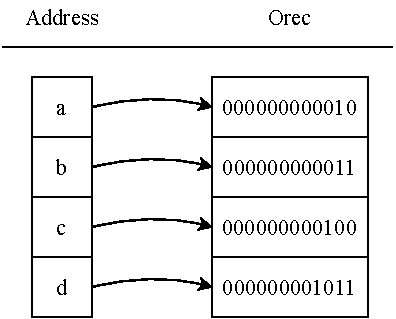
\includegraphics[width=.5\textwidth]{images/orec.pdf}
    \caption{Addresses in memory with their associated orec. Address $a$ is unlocked with version 1, Address $b$ is locked by Transaction nr. 1, Address $c$ is unlocked with version 2, and Address $d$ is locked by Transaction nr. 5}
    \label{fig:orec}
\end{figure}

\subsection{Encounter-order Transactions}
\label{subsection:etx}
Encounter-order or \textit{direct-update} transactions modify transactionally accessed memory directly. Between the transaction begins and tries to commit, all reads and writes are performed while keeping transaction-local \textit{read}, and \textit{undo} sets. The read set is used to validate during the execution of the transaction that all read-only locations' current version matches with the version recorded in the read set. The undo is used to roll back the writes upon aborting and restore the original values.

When encountering a transactional read, the location's \textit{ownership record} is fetched. The transaction needs to first check whether it already holds the lock, and in that case, the location's value can be atomically loaded, while the current version of the object is stored in the transaction's read set. In case the transaction does not hold the associated lock, it checks whether some other transaction does. If it finds the location to be locked, it can either spin or abort and retry. If the location is not locked, the value can be atomically loaded, while the current version of the object is stored in the transaction's read set.

In the case of a transactional write, firstly, the ownership record associated with the address is fetched. The transaction then must acquire the record in order to ensure that only a single transaction can write to the same location. If the lock could not be acquired (because another transaction successfully acquired it in the meanwhile), the transaction aborts. If the transaction acquired the lock, or it already holds the record, the address' current value is saved in the transaction's \textit{undo} set, and the new value is atomically stored at the address.

During the execution of the transaction, the read set must be validated to ensure that the recorded versions match the objects' current version. If a mismatch is found, there is a \textit{read-write} conflict between two transactions. In that case, another transaction modified the object that the transaction previously read; therefore, the transaction with the invalid read-set must abort.

When committing, the transaction revalidates its read-set, and if it is found to be valid, releases all locks and returns. The transaction is now considered to be committed.

Upon aborting, the transaction uses its undo-set to roll back all writes and restore the previous state as if nothing had happened. Then, it can choose to retry immediately or utilise some form of back-off, which might be useful in case of high contention.

The encounter-order approach, similar to the approaches of \cite{tl,ennals-stm}, makes committing much simpler. However, encounter-order locking has the downside of holding onto locks for a much longer time, potentially hindering performance under high contention.

\subsection{Commit-time Transactions}
\label{subsection:ctx}
Commit-time or \textit{deferred-update} transactions utilise a higher level of \textit{speculative execution} by deferring writes to commit time. During the execution, a \textit{write-set} is built, which stores the to be written values. Naturally, a \textit{read-set}, consisting of read locations and their current value, is also being book-kept, which ensures that the transaction sees valid states only.

A transactional read of an address first needs to check whether the address appears in its write-set as well, and in that case, return the latest new value in the write set. If the write set does not contain the address, the associated ownership record is fetched. If the location is found to be locked, the transaction can spin or abort. Else, the current version of the object is stored in the transaction's read set, and the location is atomically loaded.

All transactional writes are deferred to commit time; therefore, performing writes amounts to recording the address-value pair in the transaction's write-set.

During the execution of the transaction, the read-set is validated periodically by checking that the recorded version of objects matches the current version. If the read-set is found to be invalid, the transaction aborts.

When committing, all locks associated with entries in the write set must be acquired. This is done as follows: if a location in the write set appears in the read set as well (i.e. the transactional write depended on the read or vice-versa), the operation must atomically acquire the lock and validate that the version of the object at hand did not change during the execution of the transaction. If the location does not appear in the read set as well, the transaction simply acquires the associated locks. In case a lock cannot be acquired, the transaction aborts. Once all locks are acquired, the read-set is revalidated to ensure consistency, and finally, all updates are made visible using atomic stores. Afterwards, all locks are released, and the transaction is considered to be committed.

When aborting, the transaction must release all previously held locks and can be retried or can back-off based on contention.

The commit-time approach, similar to the approach of \cite{tl} and as also discussed in \cite{tl, tl2, book}, presents a much easier write operation; however, due to its speculative nature, committing is much harder, and reading involves a look-aside into the write set. For the latter, fast approaches using \textit{Bloom filters} exist, as discussed in \cite{tl2}.

Moreover, as will be presented in the Results section, commit-time transactions have an inherent limitation due to the way writes are handled. That is, only those writes will correctly be made visible, which do not depend on \textit{previous} transactional writes. In the case of transactional red-black trees, inserting a node relies heavily on intermediate rotations and recolourings, which makes commit-time transactions unsuitable or the datastructure design unnatural. In the case of skiplists, the problem disappears since swinging pointers at a certain level does not depend on earlier computed results. 

\FloatBarrier
\section{Transactional Red-Black Trees}
\label{section:trb}

One of the custom datastructures is a transactional Red-Black Tree implementation that is used to evaluate the performance of the proposed STM versions and demonstrate the ease of transactional datastructure design.

\textit{Binary trees} are tree-graphs with a root in which each node has at most two children. A \textit{binary search tree} (or BST for short) is a type of search datastructure built on top of binary trees. In a BST, each node is an object that contains \texttt{left-child}, \texttt{right-child} and \texttt{parent} pointers to other nodes, and a \texttt{key} attribute. Keys are stored with the condition that each node's key must be larger than any key in its left subtree and smaller than any key in its right sub-tree, or in other words, flattening the tree gives an increasing sequence of keys. In a binary search tree, the operations of search, insertion and deletion run in $\mathcal{O}(\text{log n})$ time in the average case; however, in the worst-case, these datastructures offer no greater performance than linked-lists with $\mathcal{O}(n)$ time\cite{introalg}. The reason behind this is that BSTs do not \textit{balance} themselves after the tree is modified; therefore, successive insertion of strictly smaller or larger elements will result in a linked-list-like structure starting at the root, which can be seen in Figure \ref{fig:bst}b.

%\renewcommand{\thefigure}{1a-1b}
\begin{figure}[!htb]
    \centering
    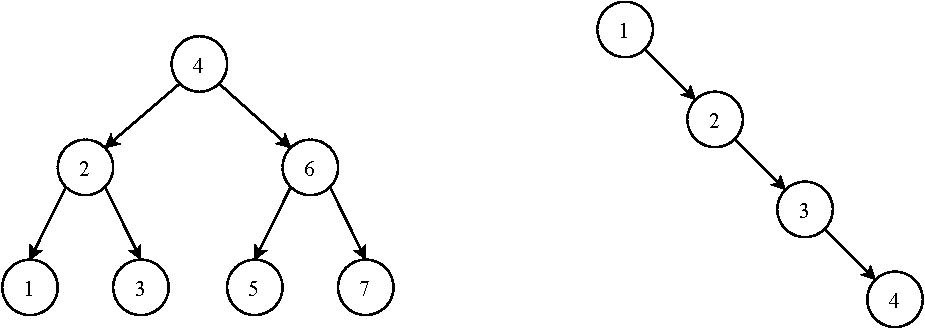
\includegraphics[width=.9\textwidth]{bst.pdf}
    \caption{a) balanced BST b) unbalanced BST}
    \label{fig:bst}
\end{figure}

Red-Black trees are a type of \textit{self-balancing} binary search tree that aim to solve the previously mentioned performance issue, permitting $\mathcal{O}(\text{log n})$ worst-case search, insertion and deletion complexity\cite{introalg}. A binary tree is considered to be balanced if the height of each nodes' left and right sub-tree differ by no more than one. The height of a binary tree is defined as the length of the longest possible path from the root to a leaf node (i.e. a node with no children).

\begin{figure}[!htb]
    \centering
    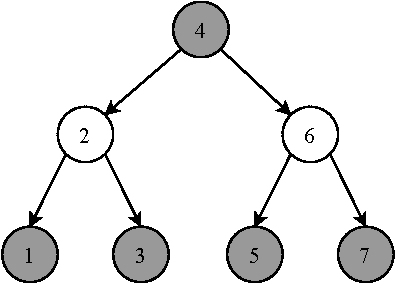
\includegraphics[width=.4\textwidth]{rbt.pdf}
    \caption{A red-black tree with shaded black and unshaded red nodes}
    \label{fig:rbt}
\end{figure}

In a red-black tree, compared to binary search trees, each node has an extra attribute, its \texttt{colour}. Each node is coloured either red or black, which, along with some local \text{rotation} operations, ensure that the tree remains balanced after insertion and deletion. The tree is painted in such a way that the following properties hold\cite{introalg}:

\begin{enumerate}
    \item Every node is painted either red or black
    \item The root and leaf nodes are black
    \item Every red node's children must be black
    \item From each node to its descendant leaves, all paths contain the same number of black nodes
\end{enumerate}

In binary search trees, the root's parent and the leaf nodes' left and right child pointers point to \texttt{NIL} (i.e. to nothing). By convention, in a red-black tree \textit{T}, a single sentinel node \textit{T.nil} is used to represent pointers to \texttt{NIL} which is always coloured black. This node has the same properties as any other node in the tree but with arbitrary key and left-right pointers. This implies that the leaf nodes of a red-black tree are always a single sentinel node; moreover, that the second part of property (2) is always ensured.

Inserting a key into a binary search tree can be summarised as follows. Start at the root of the tree and perform the following until the current node pointer is \texttt{NIL}: if the current node pointer is \texttt{NIL} insert the node at that position. If the current node is not null and the key we wish to insert is smaller than the current node's key, move the current node pointer to the left; else, move it to the right. This algorithm modifies the tree structure, which may or may not violate the properties of a red-black tree. These properties, which might be violated, are namely that the root needs to be black and that a red node cannot have red children. Therefore, when inserting keys into a red-black tree, the tree may need to be repainted, and the tree structure may need to be modified. Modifying the tree structure relies on local \textit{rotations} which are illustrated in Figure \ref{fig:rotate}.

\begin{figure}[!htb]
    \centering
    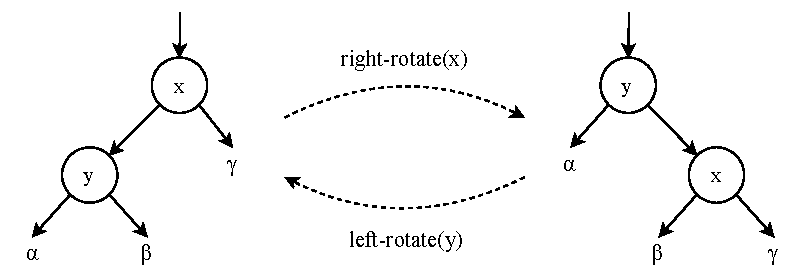
\includegraphics[width=.9\textwidth]{rotate.pdf}
    \caption{Rotation operations on binary search trees}
    \label{fig:rotate}
\end{figure}

One promising aspect of transactional datastructure design and one reason for choosing red-black trees is the simplicity involved in crafting them compared to the lock-based or lock-free approaches. Inserting and deleting keys in a red-black tree involves a \textit{rebalancing} or \textit{fixup} method compared to simple binary search trees, which makes the number of local rotations needed not known in advance. The lock-based approach would have difficulties creating a cycle-free acquisition order\cite{book}, and a lock-free approach\cite{ma, lock-free-rb, wait-free-rb} would involve modifying multiple locations at once. With transactions, the complexity of crafting such datastructure reduces to merely specifying which method needs to execute atomically, and the runtime environment will take care of the rest, which, arguably, also makes the process of crafting such datastructures more accessible and less prone to mistakes. 

To demonstrate the simplicity regarding transactional datastructure design, consider as an example the insertion algorithm described in Algorithm \ref{alg:insert}, and its transactional translation in C++ in Figures  \ref{fig:tx_insert}. The algorithm, which inserts node $z$ with key $k$ into a red-black tree $T$, can be roughly summarised as follows, while, for the sake of simplicity, the description of the fixup method responsible for repainting and performing rotations on the tree is omitted. Firstly, pointers $y$ and $x$ are initialised to nil and the root of the tree in this order. While $x$ does not point to nil, $y$ is swung to $x$ (this pointer keeps track of the parent of the new node $z$), and based on the new node $z$'s key, $x$ is swung either to its left or right child pointer. After the location of the new node is found, its parent pointer is assigned $y$. If the parent pointer is still nil, the tree was empty; therefore, the root is assigned the new node. If the tree was not empty, depending on the key of $z$, the parent node's left or right child is assigned $z$. Finally, the new node is initialised with nil left and right child pointers and the colour red.

In order to "transactionalise" this algorithm, one would need to specify which lines should execute atomically. In pseudocode, this is usually marked as an \texttt{atomic \{...\}} block wrapping the statements in the method. Provided
that compiler support exists for such, the atomic block would be parsed with a transaction initialisation in the beginning and \textit{read} statements in the form \texttt{int a = *b;} replaced with \texttt{int a = read(b);} and \textit{write} statements in the form \texttt{A = b;} replaced with \texttt{write(\&A, b);}. Here, the functions \texttt{T *read(T *)} and \texttt{void write(T *, T)} refer to the transactional interface described in Section \ref{subsec:stm_impl}. Such a translation of the sequential method can be seen in Figure \ref{fig:tx_insert}.

The method \texttt{void tx\_rb\_insert(Node<T> *)} is a member of the class\\ \texttt{TransactionalRBTree<T>} and operates on pointers to \texttt{Node<T>} objects. Notable differences to Algorithm \ref{alg:insert} are line 2 which set up a new transaction as described in Section \ref{subsec:stm_impl}, line 6 which starts the transaction, and line 29 which commits it. The atomic block (i.e. statements that should execute atomically) is placed in a \texttt{try-catch} block which is retried until the transaction is able to commit. All reads are replaced by a method calls to \texttt{Tx.read()} and writes are replaced by calls to \texttt{Tx.write()}. In case the transaction fails, i.e. during the insertion procedure some inconsistencies are encountered, all methods throw an \texttt{AbortException} which is caught by the \texttt{catch} block. The transaction then aborts itself and is retried.

\begin{algorithm}
\caption{RB-Insert(T, z)}
\label{alg:insert}
\begin{algorithmic}[1]
    \State y $\gets$ T.nil
    \State x $\gets$ T.root
    \While {x $\neq$ T.nil}
        \State y $\gets$ x
        \If{z.key $<$ x.key}
            \State x $\gets$ x.left
        \Else 
            \State x $\gets$ x.right
        \EndIf
    \EndWhile
    \State z.p $\gets$ y
    \If{y = T.nil}
        \State T.root $\gets$ z
    \ElsIf{z.key $<$ y.key}
        \State y.left $\gets$ z
    \Else
        \State y.right $\gets$ z
    \EndIf
    \State z.left $\gets$ T.nil
    \State z.right $\gets$ T.nil
    \State z.color $\gets$ RED
    \State \Call{RB-Insert-Fixup}{T, z}
\end{algorithmic}
\end{algorithm}

\begin{figure}[!htb]
\begin{lstlisting}[language=C++, escapeinside=``]
template<class T> 
void tx_rb_insert(Node<T> *z) {
    Transaction Tx;
    bool done = false;
    while (!done) {
        try {
            Tx.begin();

            Node<T> *y = Tx.read(&nil), *n = y;
            Node<T> *x = Tx.read(&root);
        
            while (x != n) {
                y = x;
                if (z->key < Tx.read(&x->key))
                    x = Tx.read(&x->left);
                else 
                    x = Tx.read(&x->right);
            }
            Tx.write(&z->parent, y);
            
            if (y == n) 
                Tx.write(&root, z);
            else if (z->key < Tx.read(&y->key)) 
                Tx.write(&y->left, z);
            else Tx.write(&y->right, z);
        
            Tx.write(&z->left, nil);
            Tx.write(&z->right, nil);
            Tx.write(&z->colour, RED);
        
            tx_rb_insert_fixup(z);
            done = Tx.commit();
        }
        catch(AbortException&) {
            Tx.abort();
            done = false;
        }
    }
}
\end{lstlisting}
\caption{Transactional insertion into a Red-Black Tree}
\label{fig:tx_insert}
\end{figure}

\FloatBarrier
\section{Transactional Skiplists}
\label{section:skip}

Skiplists are probabilistic datastructures similar in nature to balanced trees, proposed by William Pugh in 1990\cite{pugh-skiplist}. Skiplists can be thought of as linked-lists in which nodes are equipped with additional pointers to other nodes further into the list to allow for more efficient searching. They exhibit $\mathcal{O}$(log n) search, insert and delete average-case complexities and $\mathcal{O}$(n) worst-case complexities, similar to binary search trees. 

Skiplists consist of linked nodes of a certain \textit{height}, where each node with height $h$ contains $h$ forward pointers to other nodes. The height of a node is chosen with a certain probability $p$ (usually chosen to be $1/2$ or $1/4$ etc.). In case when $p = 1/2$, $50\%$ of nodes will have height $1$, $25\%$ of nodes will have height $2$, etc. Skiplists consist of \textit{levels} with level $0$ being the uppermost one in Figure \ref{fig:skiplist}, and the last level being the bottom one, which essentially acts as a conventional linked-list. The maximum level is usually capped at $\log_{1/p}$ N, where N is the upper bound on the number of elements. This means that with $p = 1/2$, up to $2^{12}$ elements can be supported with the maximum level of $12$\cite{pugh-skiplist}. Two dummy nodes, the \textit{head} and \textit{nil} represent the starting and ending points of all levels in a skiplist.

\begin{figure}[!htb]
    \centering
    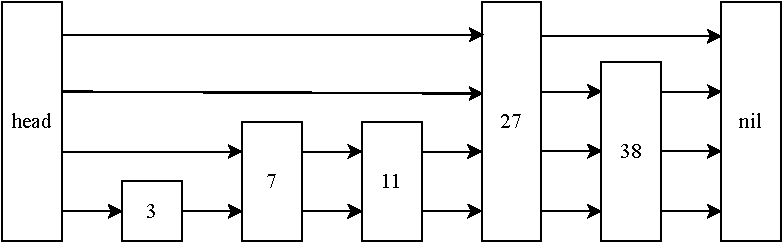
\includegraphics[width=.9\textwidth]{images/skiplist.pdf}
    \caption{Skiplist with 5 elements}
    \label{fig:skiplist}
\end{figure}

Searching in a skiplist can be summarised as follows. According to Pugh, starting at level $L(n) = \log_{1/p} n$ is most ideal, however, choosing level $0$ adds only a small constant to the complexity\cite{pugh-skiplist}. Starting at some level $n$, the key that we are searching for is compared to the key of the first forward pointer of the current node. In case the keys match, the node is found. In case the key is smaller than the next node's, we move a level down; else, we move one to the right. Until the node is found, or the current node points to nil, this procedure repeats. This algorithm is highlighted using dotted arrows in Figure \ref{fig:skip-search-insert}. 

\begin{figure}[!htb]
    \centering
    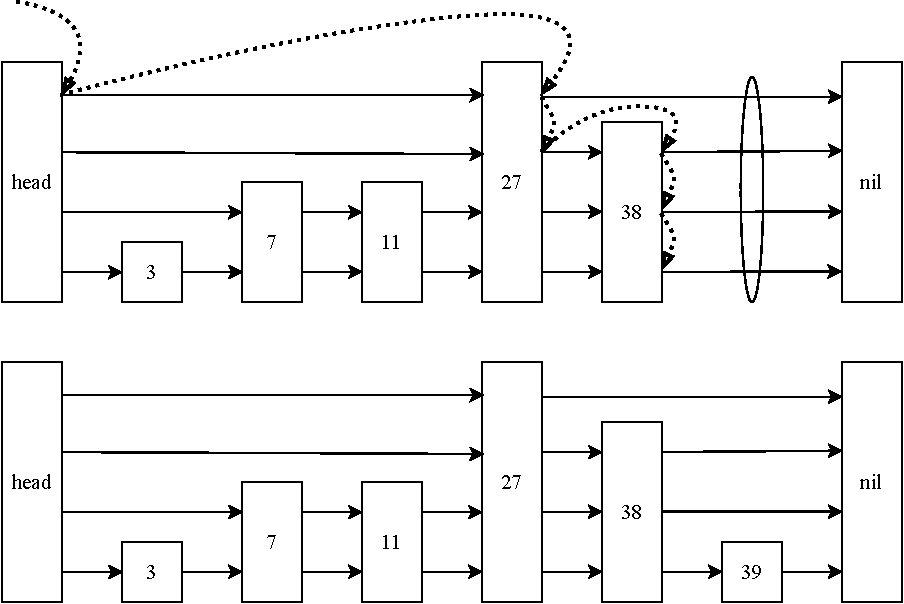
\includegraphics[width=.9\textwidth]{images/skip-search-insert.pdf}
    \caption{Inserting element $39$ with height $1$ into a skiplist. a) shows the search path to find the appropriate place on the last level. b) shows the final skiplist after insertion.}
    \label{fig:skip-search-insert}
\end{figure}

Inserting a key into a skiplist $L$, shown in Figure \ref{fig:skip-search-insert} and Algorithm \ref{alg:skip-insert}, consists of two parts. Firstly, on lines 1-8, the appropriate place of the new node needs to be found while also building an update list of pointers, which will be used to \textit{thread} the new node into the appropriate levels. Secondly, the new node needs to be inserted into the appropriate levels. If the node's random height is higher than the head's current one, the heads level is increased to match that of the new node. This is done on lines 11-17. Afterwards, a new node is allocated and threaded into the list. On line 20, the new nodes forward pointer at level $i$ is assigned the $i$th element's forward pointer in the update array. Finally, on line 21, the update array's $i$th element's forward pointers are pointed to the new node. 

\begin{algorithm}[!htb]
\caption{Skiplist-Insert(L, key)}
\label{alg:skip-insert}
\begin{algorithmic}[1]
    \State update $\gets$ [0..MaxLevel]
    \State x $\gets$ L.head
    \For{i $\gets$ L.level \textbf{downto} 0}
        \While{x.forward[i] $\neq$ nil $\land$ x.forward[i].key $<$ key}
            \State x $\gets$ x.forward[i]
        \EndWhile
        \State update[i] $\gets$ x
    \EndFor
    \State x $\gets$ x.forward[0]
    \If{x $=$ nil $\lor$ x.key $\neq$ key}
        \State h $\gets$ \Call{Get-Random-Height}{}()
        \If{h $>$ L.level}
            \For{i $\gets$ L.level$+1$ \textbf{to} h}
                \State update[i] $\gets$ L.head
            \EndFor
            \State L.level = h
        \EndIf
        \State n $\gets$ \Call{Create-Node}{h, key}
        \For{i $\gets$ 0 \textbf{to} level}
            \State n.forward[i] $\gets$ update[i].forward[i]
            \State update[i].forward[i] $\gets$ n
        \EndFor
    \EndIf
\end{algorithmic}
\end{algorithm}

Conceiving a lock-based or lock-free insertion algorithm into a skiplist would, much like with red-black trees, present a couple of difficulties that stem from the fact that the height of a node is not known in advance. A lock-based approach would need to figure out a cycle-free acquisition order of multiple node's forward pointers, and a lock-based approach would need to modify multiple locations at once when swinging the update array's forward pointers. This creates an unnatural and error-prone structure for the algorithms. Meanwhile, the transactional translation into C++, which shown in Figure \ref{fig:tx_skip_insert}, simplifies this into a naive sequential translation enclosed in a try-catch block which is retried until the transaction can commit. All reads are replaced with calls to \texttt{Tx.read()} and all writes are replaced with calls to \texttt{Tx.write()}.

\begin{figure}[!htb]
\begin{lstlisting}[language=C++]
template<class T>
void tx_skip_insert(Node<T> *n) {
    Transaction<> Tx;
    bool done = false;
    while (!done) {
        try {
            Tx.begin();
            Node<T> *curr = Tx.read(&head);
            Node<T> *update[MAX_LEVEL + 1];
            for (int i = Tx.read(&level); i >= 0; i--) {
                Node<T> *curr = Tx.read(&curr->neighbours[i]);
                while (curr && Tx.read(&curr->value) < n->value)
                    curr = Tx.read(&curr->neighbours[i]);
                update[i] = curr;
            }
            curr = Tx.read(&curr->neighbours[0]);
            if (!curr || Tx.read(&curr->value) != n->value) {
                int h = n->height;
                if (h > Tx.read(&level)) {
                    for (int i = Tx.read(&level)+1; i<h+1; i++)
                        update[i] = Tx.read(&head);
                    Tx.write(&level, h);
                }
                for (int i = 0; i <= h; i++) {
                    Tx.write(&n->neighbours[i], 
                             update[i]->neighbours[i]);
                    Tx.write(&update[i]->neighbours[i], n);
                }
            }
        }
        catch(AbortException&) {
            Tx.abort();
            done = false;
        }
    }
}
\end{lstlisting}
\caption{Transactional insertion into a Skiplist}
\label{fig:tx_skip_insert}
\end{figure}

Presented here the function \texttt{void tx\_skip\_insert(Node<T> *n)} is a member of the class \texttt{TransactionalSkiplist<T>} and is responsible for inserting a Node of type \texttt{T}.

\chapter{Evaluation}
\label{chapter:eval}
\section{Method}

In order to benchmark and measure the performance of STM versions described in Section \ref{subsec:stm_impl}, certain iterations of tests will be performed on the datastructures detailed in Section \ref{section:trb} and \ref{section:skip}. 

The tests are run on the DAS5\cite{das5}, a 6-cluster, 200-node, 16-core per node distributed system for scientific computing in the Netherlands, designed by the Advanced School of Computing and Imaging (ASCI). Of the whole network, a single node is utilised to run the test scripts. Therefore, the number of threads the tests are run on is bounded by 16, and the tests could be run on 1, 2, 4, 8 and 16 threads, respectively.

The first test, plotted in Figures \ref{fig:plots10k-insert}, \ref{fig:plots10k-speedup}, involves 10k insertions into both the Red-Black Tree and Skiplist datastructures. In this test, only insertions are performed, as the procedure for deletion is much similar and involves about the same complexity and type of internal operations. The keys that each thread inserts are determined at runtime, where each thread inserts all integers in the interval $[{i * n}, {(i + 1)n})$, where $n$ is defined as the number of total insertions over the number of threads, and $i$ is the id of the thread which ranges from 0 to 15 at the maximum. This results in storing 10k different values in the datastructure, with the actual insertion being high-contention. The same test was run using 100k and 1M insertions as well, and the results showed a very similar pattern to the 10k insertions test; therefore, it was decided to only include the latter.

In the case of the Red-Black Tree, only encounter-order transactions are utilised. Due to the nature and specific implementation details of the datastructure, the use of commit-time transactions proved unsuccessful. This is mainly due to how commit-time transactions perform their writes: namely that it records the \textit{address} of the word in memory that it later wishes to change. Consider the scenario when the first node is inserted into the datastructure. The insertion algorithm described in Section \ref{section:trb} effectively performs two steps: it swings the root pointer to the new node and paints the root black. Let $\mathcal{A}$ be the address of the root, $\mathcal{B}$ be the address of the root's colour field, and finally, $\mathcal{Z}\text{ and }\mathcal{Z}'$ be the address of the to-be-inserted node and its colour. The write-list of the commit-time transaction upon committing this single insertion contains then the following 2-tuples: $\{\langle\mathcal{A}, \mathcal{Z}\rangle , \langle\mathcal{B}, \textit{"black"}\rangle\}$. After a successful commit, however, one would find that the new root's colour is still red, and the last step, i.e. the recolouring of the root, affected the dummy node of the root and not the newly inserted node. When such dependencies of writes are included in some method, the proposed commit-time algorithm of Section \ref{subsection:ctx} yields incorrect results. On careful inspection, one might notice that this is not a problem for the insertion algorithm of the Skiplist datastructure in Section \ref{section:skip}, as inserting an element only swings pointers of nodes to the left of the newly inserted node, and those swings never depend on each other.

When performing the insertions, three measures are recorded: the mean wall-clock time of the total insertions with the standard deviation of the trial runs and the normalised speedup of each thread compared to the sequential run; finally, the mean abort rate, defined as the number of times a transaction needs to abort before successfully committing, is plotted.

In order to have a better understanding on the costs of the API operations of the transactional interface, the certain operations \texttt{begin()}, \texttt{read()}, \texttt{write()}, \texttt{commit()}, and \texttt{abort()}, are also separately timed and plotted in Figure \ref{fig:op-times}. In this test, the mean wall-clock times of the operations involving 10k insertions into a Skiplist was measured and plotted in a scaled barplot.

\section{Results}
\label{section:res}

The 10k insertions into the Red-Black Tree datastructure gave interesting results. In the first column Figure \ref{fig:plots10k-insert}, the mean wall-clock time of 10k insertions and its corresponding abort rates are plotted. As it can be seen, the execution time exhibits a logarithmic decrease until four threads, then a steady logarithmic increase as more than four threads are utilised. Similarly, for the abort rate, at $x = 4$, there is a clear inflexion point, where the slow increase in abort rate suddenly jumps, and at $x = 8$, it is about seven times as high. Due to the high abort rate and thereby slow execution time, the speedup compared to the sequential execution stops increasing at $x = 4$ and starts a drastic decrease as it can be seen on the first plot of Figure \ref{fig:plots10k-speedup}. The maximum speedup that the encounter-order algorithm could achieve was about twice as fast as the sequential execution, which is similar to what the Skiplist insertion speedup achieved when the number of threads was 4.

In the case of the Skiplist, the results obtained are much more pleasing, as the second plot of the second column in Figure \ref{fig:plots10k-insert} exhibits a rather smooth logarithmic decrease and thereby optimal scaling properties for both algorithms. As the tests performed were high-contention, the commit-time algorithm performs about twice as slow compared to the encounter-order one. As can be seen, the abort rate of the commit-time algorithm is about five times as high as that of the encounter-order algorithm when 16 threads are utilised. The speedup, as it can be seen in the second plot of Figure \ref{fig:plots10k-speedup}, compared to the sequential execution of both algorithms are about the same, with execution on 16 threads achieving a speedup of about $5.8$.

\begin{figure}[!htb]
    \centering
    \makebox[\textwidth][c]{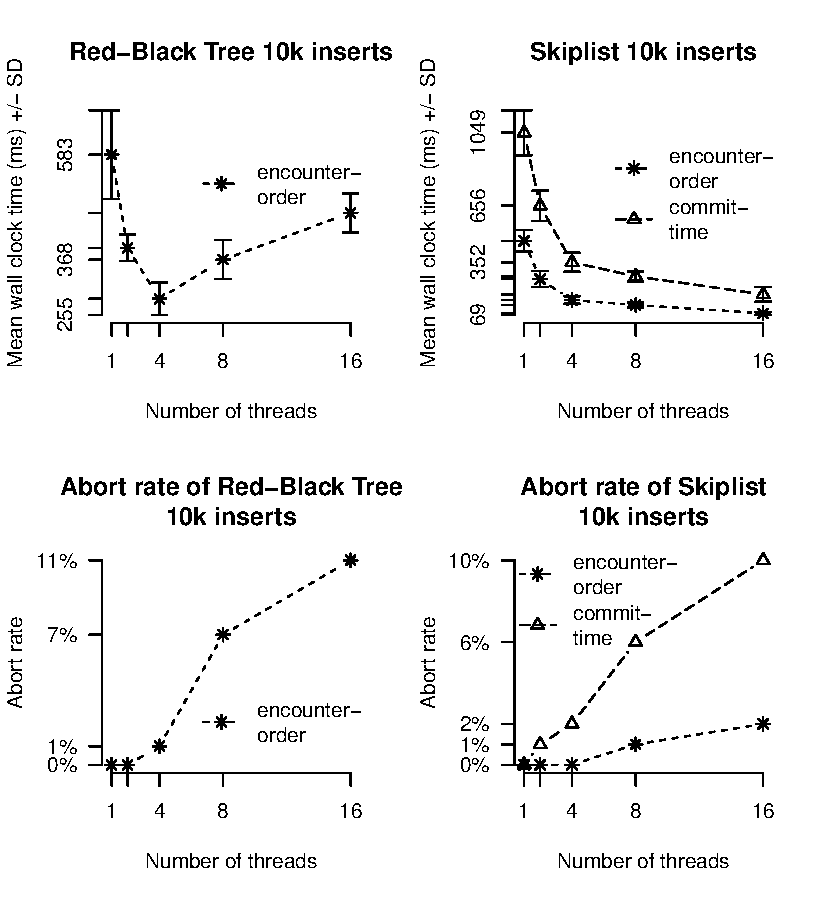
\includegraphics[width=.9\textwidth]{images/plots10k-insert-abort.pdf}}
    \vspace{-0.3cm}
    \caption{Red-Black Tree and Skiplist 10k insertion execution times using encounter-order and commit-time transactions and corresponding abort rates}
    \label{fig:plots10k-insert}
\end{figure}

\begin{figure}[!htb]
    \centering
    \makebox[\textwidth][c]{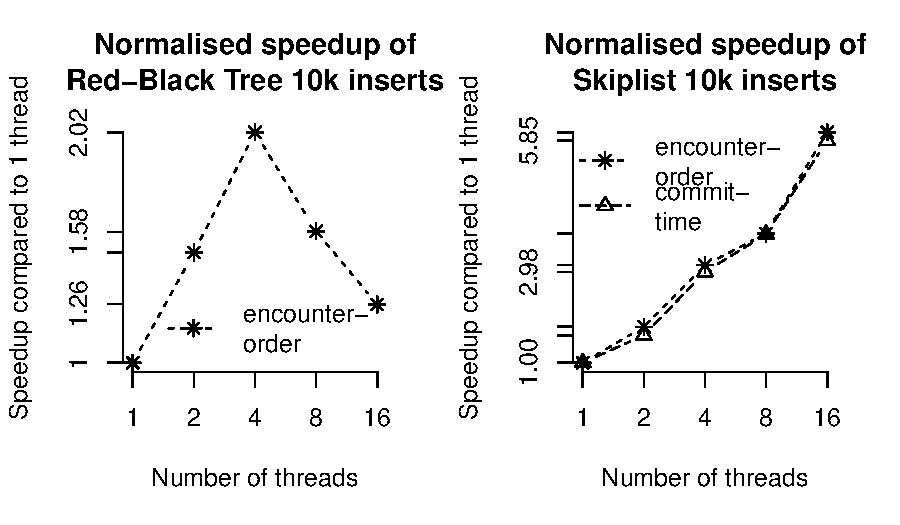
\includegraphics[width=.9\textwidth]{images/plots10k-speedup.pdf}}
    \vspace{-0.3cm}
    \caption{Red-Black Tree and Skiplist 10k insertions speedup compared to sequential execution time}
    \label{fig:plots10k-speedup}
\end{figure}

The relative execution times of the certain operations in the transactional API plotted in Figure \ref{fig:op-times}, provides no surprises, as by analysing the complexities of the algorithms described in Sections \ref{subsection:etx} and \ref{subsection:ctx}, one could have already anticipated the results. 

For the encounter-order algorithm, the \texttt{write()} operation clearly takes up more than half of all the combined execution times as it is responsible for read-set validation, lock acquisition and the atomic stores as well. Following it, the \texttt{commit()} method is the second most costly, responsible for the read-set validation and state reset. The \texttt{abort()} method takes up $7\%$ of all execution times, which is responsible for atomically storing back the original values for the locations. The \texttt{begin()} and \texttt{read()} methods have negligible time complexities, comprised mostly of simple statements and an atomic load in case of the read method. 

For the commit-time algorithm, as one could have expected, it is the \texttt{commit()} method that takes up most of the execution time. It is responsible for lock acquisition, which, due to the existence of the read-set, is in $\mathcal{O}\text{(}n^2\text{)}$; moreover, the read-set validation and atomic stores. Following are the \texttt{write()}, and \texttt{read()} methods, which both need to traverse the write-set to check whether the location is already contained and update the value or return the stored value, respectively. The methods for \texttt{begin()} and \texttt{abort()} have negligible impact on performance, as they consist mostly of simple statements of assignments.

\begin{figure}[!htb]
    \centering
    \makebox[\textwidth][c]{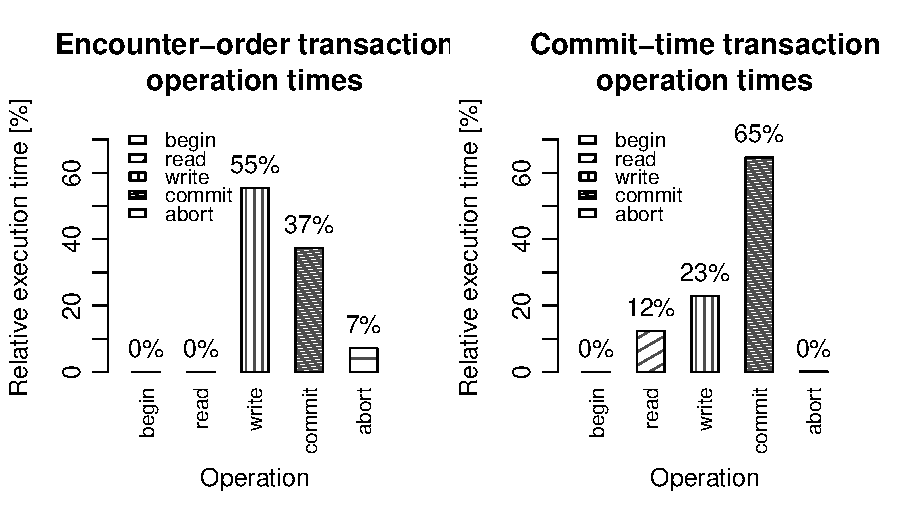
\includegraphics[width=.9\textwidth]{images/op-times.pdf}}
    \caption{Relative operation times of encounter-order and commit-time transactions}
    \label{fig:op-times}
\end{figure}

\section{Discussion}

The performance of the Red-Black Tree is not ideal, as it does not scale well to highly concurrent applications. The suboptimal scaling properties can be largely attributed to the complexity of the Red-Black Tree insertion procedure, which potentially involves a large (and initially unknown) amount of rotations and recolouring, which increases to a great extent the probability of an invalid read-set and hence the rate of aborts. This can also be confirmed by looking at the second plot in the first column of Figure \ref{fig:plots10k-insert} where the abort rate of the encounter-order algorithm is plotted.

As the encounter-order algorithm described in Section \ref{subsection:etx} is similar in nature to the STM proposed by Ennals\cite{ennals-stm}, these findings are in line with what is described by Dice and Shavit in their paper detailing the TL algorithm\cite{tl}, where the performance of encounter-order algorithms are compared. In that paper, the Red-Black Tree test using Ennals' STM version exhibited very similar properties and patterns to what is described in the previous section, matching even the infliction point at $x = 4$.

In the case of the Skiplist, the encounter-order algorithm outperforms the commit-time with about a factor of two in mean wall-clock time and with a factor of 5 in abort rate, even though the achieved speedup was relatively similar for both. This is not in line with the findings of other papers like \cite{tl, tl2}, where it is concluded that commit-time locking should be utilised in case of high contention. However, it can easily be seen that in case of high contention, the abort rate of the commit-time algorithm would drastically increase since there is a very high chance that the read-set is invalidated. This can be further confirmed by looking at the last plot of the second column, where the abort rates are plotted. In the case of executing on 16 threads, there is a difference of a factor of 5 between the abort rate of the encounter order and commit-time locking mechanisms. Encounter-order locking is considered to be a disadvantage by \cite{tl, tl2} as it holds onto locks for a much longer time. However, precisely because of this property, it has a much lower chance of aborting and could still achieve a better performance in the experiment. Moreover, the commit-time algorithm contains a lookaside into the write- and read-sets during committing, as explained in Section \ref{subsection:ctx}, which has $\mathcal{O}(n^2)$ complexity, and its read algorithm has linear time complexity. Compared to the encounter-order algorithm, which has $\mathcal{O}(1)$ read and linear time commit complexities, it is easy to see how it can overperform the commit-time version. We can conclude that the disadvantage of the encounter-order algorithm, namely that it holds onto locks for a much longer time, is still preferable to the complexities introduced in the commit-time algorithm in high-contention situations.

\chapter{Conclusion}
The paper set out to describe the intricacies of software transaction memory and its main approaches, namely the non-blocking and lock-based versions. In doing so, concurrent datastructure design emerged as a potential area where the transactional techniques could be applied successfully. By using the transactional approach to create concurrent datastructures, the process of crafting them moves away from the use of error-prone and difficult-to-reason-about lock-based and unnaturally structured lock-free algorithms to much more accessible and straightforward ones. Similarly to findings described in \cite{is-tx-easier}, this paper could also empirically conclude that apart from a few quirks in notation, writing concurrent transactional algorithms are not very different from their sequential counterpart while also being concurrent and correct. Results showed that the commit-time lock-based transactions could only be applied, without imposing an unnatural design on the datastructure itself, in cases where there are no direct dependencies between the writes. This is attributed to the fact that the commit-time transaction records its writes as a list of (address, value) 2-tuples that are oblivious to whether one write depends on the result of others. The encounter-order approach, however, can safely be applied in all situations; moreover, as opposed to findings of papers like \cite{tl, tl2}, under high-contention, it even outperforms its commit-time counterpart. This is due to the fact that under high contention, the commit-time transaction has a much higher abort rate as its read-set is invalidated more and more frequently, and its operations have worse time complexities, which hinders its performance. Further research could investigate how word-based commit-time transactions can overcome their limitations concerning the dependencies between their writes. Moreover, many popular datastructures whose internal complexities create rather complex lock-based or lock-free implementations could be explored and show that its transactional version is rather straightforward. Shifting to transactional design in place of the lock-based or lock-free style could be considered a viable alternative by creating an accessible abstraction to deal with concurrency.

\printbibliography[heading=bibintoc]

\end{document}